\documentclass[]{article}
\usepackage{lmodern}
\usepackage{amssymb,amsmath}
\usepackage{ifxetex,ifluatex}
\usepackage{fixltx2e} % provides \textsubscript
\ifnum 0\ifxetex 1\fi\ifluatex 1\fi=0 % if pdftex
  \usepackage[T1]{fontenc}
  \usepackage[utf8]{inputenc}
\else % if luatex or xelatex
  \ifxetex
    \usepackage{mathspec}
  \else
    \usepackage{fontspec}
  \fi
  \defaultfontfeatures{Ligatures=TeX,Scale=MatchLowercase}
\fi
% use upquote if available, for straight quotes in verbatim environments
\IfFileExists{upquote.sty}{\usepackage{upquote}}{}
% use microtype if available
\IfFileExists{microtype.sty}{%
\usepackage{microtype}
\UseMicrotypeSet[protrusion]{basicmath} % disable protrusion for tt fonts
}{}
\usepackage[margin=1in]{geometry}
\usepackage{hyperref}
\hypersetup{unicode=true,
            pdftitle={Reproducible Research: Peer Assessment 1},
            pdfborder={0 0 0},
            breaklinks=true}
\urlstyle{same}  % don't use monospace font for urls
\usepackage{color}
\usepackage{fancyvrb}
\newcommand{\VerbBar}{|}
\newcommand{\VERB}{\Verb[commandchars=\\\{\}]}
\DefineVerbatimEnvironment{Highlighting}{Verbatim}{commandchars=\\\{\}}
% Add ',fontsize=\small' for more characters per line
\usepackage{framed}
\definecolor{shadecolor}{RGB}{248,248,248}
\newenvironment{Shaded}{\begin{snugshade}}{\end{snugshade}}
\newcommand{\KeywordTok}[1]{\textcolor[rgb]{0.13,0.29,0.53}{\textbf{#1}}}
\newcommand{\DataTypeTok}[1]{\textcolor[rgb]{0.13,0.29,0.53}{#1}}
\newcommand{\DecValTok}[1]{\textcolor[rgb]{0.00,0.00,0.81}{#1}}
\newcommand{\BaseNTok}[1]{\textcolor[rgb]{0.00,0.00,0.81}{#1}}
\newcommand{\FloatTok}[1]{\textcolor[rgb]{0.00,0.00,0.81}{#1}}
\newcommand{\ConstantTok}[1]{\textcolor[rgb]{0.00,0.00,0.00}{#1}}
\newcommand{\CharTok}[1]{\textcolor[rgb]{0.31,0.60,0.02}{#1}}
\newcommand{\SpecialCharTok}[1]{\textcolor[rgb]{0.00,0.00,0.00}{#1}}
\newcommand{\StringTok}[1]{\textcolor[rgb]{0.31,0.60,0.02}{#1}}
\newcommand{\VerbatimStringTok}[1]{\textcolor[rgb]{0.31,0.60,0.02}{#1}}
\newcommand{\SpecialStringTok}[1]{\textcolor[rgb]{0.31,0.60,0.02}{#1}}
\newcommand{\ImportTok}[1]{#1}
\newcommand{\CommentTok}[1]{\textcolor[rgb]{0.56,0.35,0.01}{\textit{#1}}}
\newcommand{\DocumentationTok}[1]{\textcolor[rgb]{0.56,0.35,0.01}{\textbf{\textit{#1}}}}
\newcommand{\AnnotationTok}[1]{\textcolor[rgb]{0.56,0.35,0.01}{\textbf{\textit{#1}}}}
\newcommand{\CommentVarTok}[1]{\textcolor[rgb]{0.56,0.35,0.01}{\textbf{\textit{#1}}}}
\newcommand{\OtherTok}[1]{\textcolor[rgb]{0.56,0.35,0.01}{#1}}
\newcommand{\FunctionTok}[1]{\textcolor[rgb]{0.00,0.00,0.00}{#1}}
\newcommand{\VariableTok}[1]{\textcolor[rgb]{0.00,0.00,0.00}{#1}}
\newcommand{\ControlFlowTok}[1]{\textcolor[rgb]{0.13,0.29,0.53}{\textbf{#1}}}
\newcommand{\OperatorTok}[1]{\textcolor[rgb]{0.81,0.36,0.00}{\textbf{#1}}}
\newcommand{\BuiltInTok}[1]{#1}
\newcommand{\ExtensionTok}[1]{#1}
\newcommand{\PreprocessorTok}[1]{\textcolor[rgb]{0.56,0.35,0.01}{\textit{#1}}}
\newcommand{\AttributeTok}[1]{\textcolor[rgb]{0.77,0.63,0.00}{#1}}
\newcommand{\RegionMarkerTok}[1]{#1}
\newcommand{\InformationTok}[1]{\textcolor[rgb]{0.56,0.35,0.01}{\textbf{\textit{#1}}}}
\newcommand{\WarningTok}[1]{\textcolor[rgb]{0.56,0.35,0.01}{\textbf{\textit{#1}}}}
\newcommand{\AlertTok}[1]{\textcolor[rgb]{0.94,0.16,0.16}{#1}}
\newcommand{\ErrorTok}[1]{\textcolor[rgb]{0.64,0.00,0.00}{\textbf{#1}}}
\newcommand{\NormalTok}[1]{#1}
\usepackage{graphicx,grffile}
\makeatletter
\def\maxwidth{\ifdim\Gin@nat@width>\linewidth\linewidth\else\Gin@nat@width\fi}
\def\maxheight{\ifdim\Gin@nat@height>\textheight\textheight\else\Gin@nat@height\fi}
\makeatother
% Scale images if necessary, so that they will not overflow the page
% margins by default, and it is still possible to overwrite the defaults
% using explicit options in \includegraphics[width, height, ...]{}
\setkeys{Gin}{width=\maxwidth,height=\maxheight,keepaspectratio}
\IfFileExists{parskip.sty}{%
\usepackage{parskip}
}{% else
\setlength{\parindent}{0pt}
\setlength{\parskip}{6pt plus 2pt minus 1pt}
}
\setlength{\emergencystretch}{3em}  % prevent overfull lines
\providecommand{\tightlist}{%
  \setlength{\itemsep}{0pt}\setlength{\parskip}{0pt}}
\setcounter{secnumdepth}{0}
% Redefines (sub)paragraphs to behave more like sections
\ifx\paragraph\undefined\else
\let\oldparagraph\paragraph
\renewcommand{\paragraph}[1]{\oldparagraph{#1}\mbox{}}
\fi
\ifx\subparagraph\undefined\else
\let\oldsubparagraph\subparagraph
\renewcommand{\subparagraph}[1]{\oldsubparagraph{#1}\mbox{}}
\fi

%%% Use protect on footnotes to avoid problems with footnotes in titles
\let\rmarkdownfootnote\footnote%
\def\footnote{\protect\rmarkdownfootnote}

%%% Change title format to be more compact
\usepackage{titling}

% Create subtitle command for use in maketitle
\newcommand{\subtitle}[1]{
  \posttitle{
    \begin{center}\large#1\end{center}
    }
}

\setlength{\droptitle}{-2em}

  \title{Reproducible Research: Peer Assessment 1}
    \pretitle{\vspace{\droptitle}\centering\huge}
  \posttitle{\par}
    \author{}
    \preauthor{}\postauthor{}
    \date{}
    \predate{}\postdate{}
  

\begin{document}
\maketitle

\subsection{Loading and preprocessing the
data}\label{loading-and-preprocessing-the-data}

\begin{enumerate}
\def\labelenumi{\arabic{enumi}.}
\tightlist
\item
  First load data we load the data from ``activity.csv'' and store into
  a Dataframe called ``activity'':
\end{enumerate}

\begin{Shaded}
\begin{Highlighting}[]
\NormalTok{activity<-}\KeywordTok{read.csv}\NormalTok{(}\StringTok{"activity.csv"}\NormalTok{)}
\end{Highlighting}
\end{Shaded}

\subsection{What is mean total number of steps taken per
day?}\label{what-is-mean-total-number-of-steps-taken-per-day}

In order to plot a histogram of daily steps, we aggregate the steps by
day using the function ``aggregate'' and apply appropriate column names:

\begin{Shaded}
\begin{Highlighting}[]
\CommentTok{#Calculate average steps per 5-min interval using 'aggregate' and store it in 'activity_daily' dataframe}
\NormalTok{activity_daily<-}\KeywordTok{aggregate}\NormalTok{(activity}\OperatorTok{$}\NormalTok{steps,}\DataTypeTok{by=}\KeywordTok{list}\NormalTok{(}\KeywordTok{as.Date}\NormalTok{(activity}\OperatorTok{$}\NormalTok{date)),sum)}

\CommentTok{#Give appropriate coumn names for newly created datafrae}
\KeywordTok{colnames}\NormalTok{(activity_daily)<-}\KeywordTok{c}\NormalTok{(}\StringTok{"date"}\NormalTok{,}\StringTok{"dailysteps"}\NormalTok{)}
\end{Highlighting}
\end{Shaded}

From the aggregated data of \textbf{activity\_daily} we create a
frequency plot (histogram) if daily steps, like so:

\begin{Shaded}
\begin{Highlighting}[]
\KeywordTok{hist}\NormalTok{(activity_daily}\OperatorTok{$}\NormalTok{dailysteps, }\DataTypeTok{xlab=}\StringTok{"Daily Steps"}\NormalTok{, }\DataTypeTok{main =} \StringTok{"Daily Steps Frequency Plot"}\NormalTok{)}
\end{Highlighting}
\end{Shaded}

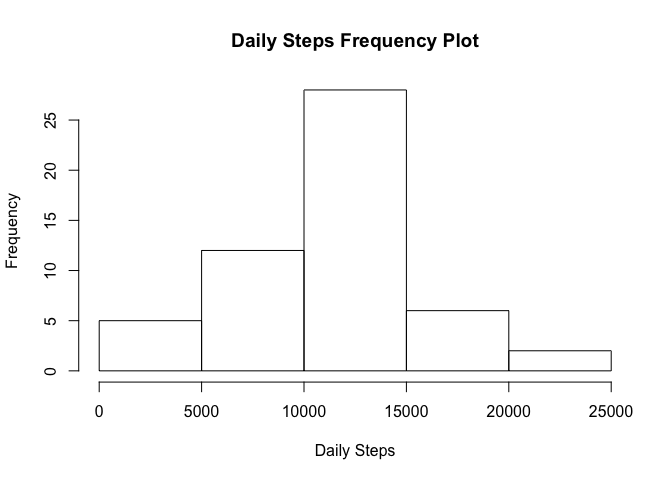
\includegraphics{PA1_template_files/figure-latex/histogram plot-1.pdf}

We can also see figure out the \emph{mean} ``daily steps'' (we remove NA
values):

\begin{Shaded}
\begin{Highlighting}[]
\KeywordTok{mean}\NormalTok{(activity_daily}\OperatorTok{$}\NormalTok{dailysteps, }\DataTypeTok{na.rm =} \OtherTok{TRUE}\NormalTok{)}
\end{Highlighting}
\end{Shaded}

\begin{verbatim}
## [1] 10766.19
\end{verbatim}

and the \emph{median} daily steps is:

\begin{Shaded}
\begin{Highlighting}[]
\KeywordTok{median}\NormalTok{(activity_daily}\OperatorTok{$}\NormalTok{dailysteps, }\DataTypeTok{na.rm =} \OtherTok{TRUE}\NormalTok{)}
\end{Highlighting}
\end{Shaded}

\begin{verbatim}
## [1] 10765
\end{verbatim}

\subsection{What is the average daily activity
pattern?}\label{what-is-the-average-daily-activity-pattern}

First we create a new data frame with average steps for each 5-min
interval and assgin relevant names:

\begin{Shaded}
\begin{Highlighting}[]
\NormalTok{stepsperint<-}\KeywordTok{aggregate}\NormalTok{(activity}\OperatorTok{$}\NormalTok{steps,}\DataTypeTok{by=}\KeywordTok{list}\NormalTok{(activity}\OperatorTok{$}\NormalTok{interval),mean,}\DataTypeTok{na.rm=}\OtherTok{TRUE}\NormalTok{)}
\KeywordTok{colnames}\NormalTok{(stepsperint)<-}\KeywordTok{c}\NormalTok{(}\StringTok{"interval"}\NormalTok{,}\StringTok{"averagesteps"}\NormalTok{)}
\end{Highlighting}
\end{Shaded}

Then we plot a time series for the average steps for each interval of
the day:

\begin{Shaded}
\begin{Highlighting}[]
\KeywordTok{plot}\NormalTok{(stepsperint}\OperatorTok{$}\NormalTok{interval,stepsperint}\OperatorTok{$}\NormalTok{averagesteps,}\DataTypeTok{type=}\StringTok{'l'}\NormalTok{,}\DataTypeTok{xlab=}\StringTok{"5 min Interval"}\NormalTok{,}\DataTypeTok{ylab=}\StringTok{"Average Steps per Interval"}\NormalTok{)}
\end{Highlighting}
\end{Shaded}

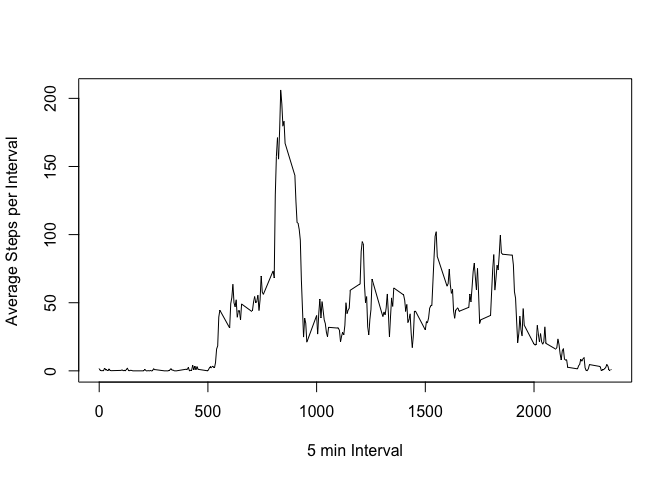
\includegraphics{PA1_template_files/figure-latex/plot for average steps per internval-1.pdf}

We can see that the maximum average steps per day happens in the morning
at:

\begin{Shaded}
\begin{Highlighting}[]
\NormalTok{stepsperint}\OperatorTok{$}\NormalTok{interval[stepsperint}\OperatorTok{$}\NormalTok{averagesteps}\OperatorTok{==}\KeywordTok{max}\NormalTok{(stepsperint}\OperatorTok{$}\NormalTok{averagesteps)]}
\end{Highlighting}
\end{Shaded}

\begin{verbatim}
## [1] 835
\end{verbatim}

\subsection{Imputing missing values}\label{imputing-missing-values}

There are following number of missing values:

\begin{Shaded}
\begin{Highlighting}[]
\KeywordTok{sum}\NormalTok{(}\KeywordTok{is.na}\NormalTok{(activity}\OperatorTok{$}\NormalTok{steps))}
\end{Highlighting}
\end{Shaded}

\begin{verbatim}
## [1] 2304
\end{verbatim}

Where there's an ``NA'' value, we're going to replace it with the
average steps of that specific 5-minute interval obtained in the
previous section:

\begin{Shaded}
\begin{Highlighting}[]
\NormalTok{##create a clone of loaded csv data}
\NormalTok{activityNoNA<-activity}
\NormalTok{##replace NAs with average steps for that specific 5-min interval calculated in the previous section}
\NormalTok{activityNoNA}\OperatorTok{$}\NormalTok{steps<-}\KeywordTok{ifelse}\NormalTok{(}\KeywordTok{is.na}\NormalTok{(activityNoNA}\OperatorTok{$}\NormalTok{steps),stepsperint}\OperatorTok{$}\NormalTok{averagesteps[}\KeywordTok{match}\NormalTok{(activityNoNA}\OperatorTok{$}\NormalTok{interval,stepsperint}\OperatorTok{$}\NormalTok{interval)],activityNoNA}\OperatorTok{$}\NormalTok{steps)}
\end{Highlighting}
\end{Shaded}

In order to plot a histogram with new data (with no NAs), we sum steps
by day:

\begin{Shaded}
\begin{Highlighting}[]
\NormalTok{activityNoNA_daily<-}\KeywordTok{aggregate}\NormalTok{(activityNoNA}\OperatorTok{$}\NormalTok{steps,}\DataTypeTok{by=}\KeywordTok{list}\NormalTok{(}\KeywordTok{as.Date}\NormalTok{(activityNoNA}\OperatorTok{$}\NormalTok{date)),sum)}
\KeywordTok{colnames}\NormalTok{(activityNoNA_daily)<-}\KeywordTok{c}\NormalTok{(}\StringTok{"date"}\NormalTok{,}\StringTok{"dailysteps"}\NormalTok{)}
\end{Highlighting}
\end{Shaded}

With the new aggregated data, we plot histogram of Daily Steps:

\begin{Shaded}
\begin{Highlighting}[]
\KeywordTok{hist}\NormalTok{(activityNoNA_daily}\OperatorTok{$}\NormalTok{dailysteps, }\DataTypeTok{xlab=}\StringTok{"Daily Steps"}\NormalTok{, }\DataTypeTok{main =} \StringTok{"Daily Steps Frequency Plot "}\NormalTok{)}
\end{Highlighting}
\end{Shaded}

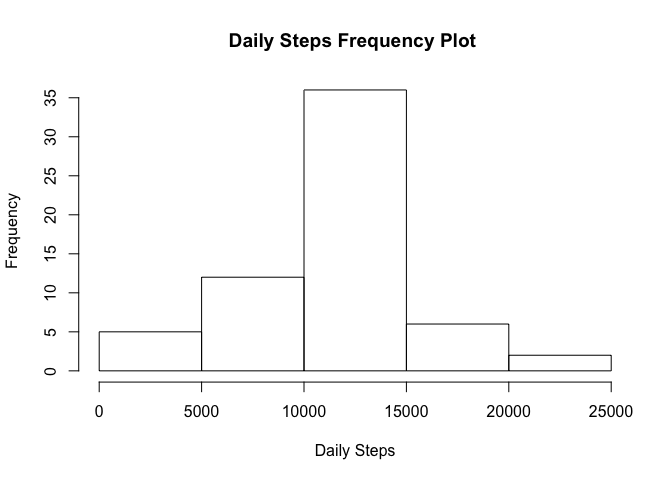
\includegraphics{PA1_template_files/figure-latex/plot histogram with new data-1.pdf}

the new data has a \emph{mean} of steps:

\begin{Shaded}
\begin{Highlighting}[]
\KeywordTok{mean}\NormalTok{(activityNoNA_daily}\OperatorTok{$}\NormalTok{dailysteps)}
\end{Highlighting}
\end{Shaded}

\begin{verbatim}
## [1] 10766.19
\end{verbatim}

And a \emph{median} of:

\begin{Shaded}
\begin{Highlighting}[]
\KeywordTok{median}\NormalTok{(activityNoNA_daily}\OperatorTok{$}\NormalTok{dailysteps)}
\end{Highlighting}
\end{Shaded}

\begin{verbatim}
## [1] 10766.19
\end{verbatim}

TODO

\subsection{Are there differences in activity patterns between weekdays
and
weekends?}\label{are-there-differences-in-activity-patterns-between-weekdays-and-weekends}

TODO

\begin{Shaded}
\begin{Highlighting}[]
\CommentTok{#discern whether it's a weekday or weekend and store into a vector ("DayType")}
\NormalTok{daytype<-}\KeywordTok{ifelse}\NormalTok{(}\KeywordTok{weekdays}\NormalTok{(}\KeywordTok{as.Date}\NormalTok{(activityNoNA}\OperatorTok{$}\NormalTok{date))}\OperatorTok{==}\StringTok{"Sunday"}\OperatorTok{|}\KeywordTok{weekdays}\NormalTok{(}\KeywordTok{as.Date}\NormalTok{(activityNoNA}\OperatorTok{$}\NormalTok{date))}\OperatorTok{==}\StringTok{"Saturday"}\NormalTok{,}\StringTok{"weekend"}\NormalTok{,}\StringTok{"weekday"}\NormalTok{)}

\CommentTok{#Merge DayType vector with activityNoNA}
\NormalTok{activityNoNA_daytype<-}\KeywordTok{data.frame}\NormalTok{(activityNoNA,daytype)}

\CommentTok{#Sum (and group) steps by DayType and Interval}
\NormalTok{stepsperint_daytype<-}\KeywordTok{aggregate}\NormalTok{(activityNoNA_daytype}\OperatorTok{$}\NormalTok{steps,}\DataTypeTok{by=}\KeywordTok{list}\NormalTok{(activityNoNA_daytype}\OperatorTok{$}\NormalTok{interval,activityNoNA_daytype}\OperatorTok{$}\NormalTok{daytype),sum)}

\CommentTok{#Give new table (stepsperint_daytype) appropriate column}
\KeywordTok{colnames}\NormalTok{(stepsperint_daytype)<-}\KeywordTok{c}\NormalTok{(}\StringTok{"interval"}\NormalTok{,}\StringTok{"daytype"}\NormalTok{,}\StringTok{"steps"}\NormalTok{)}

\CommentTok{#Plot steps per 5-min interval, split by day type (using Lattice library):}
\KeywordTok{library}\NormalTok{(lattice)}
\KeywordTok{xyplot}\NormalTok{(steps}\OperatorTok{~}\NormalTok{interval}\OperatorTok{|}\StringTok{ }\NormalTok{daytype,}\DataTypeTok{data=}\NormalTok{stepsperint_daytype, }\DataTypeTok{type=}\StringTok{"l"}\NormalTok{)}
\end{Highlighting}
\end{Shaded}

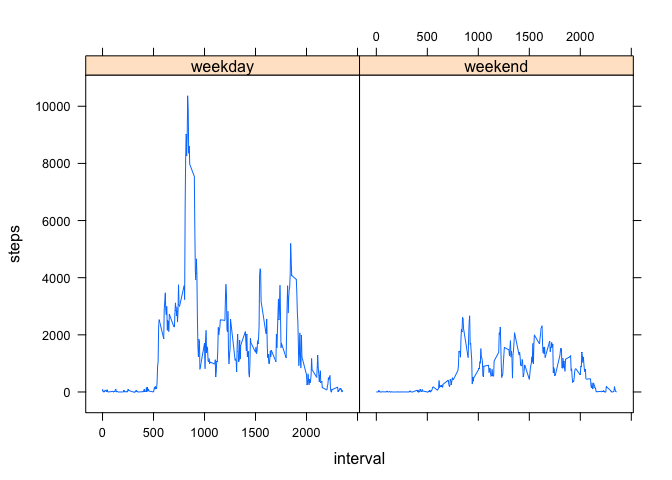
\includegraphics{PA1_template_files/figure-latex/DataWithDayType-1.pdf}


\end{document}
